\documentclass[12pt, a4paper, simple]{eskdtext}

\usepackage{hyperref}
\usepackage{env}
\usepackage{_sty/gpi_lst}
\usepackage{_sty/gpi_toc}
\usepackage{_sty/gpi_t}
\usepackage{_sty/gpi_p}
\usepackage{_sty/gpi_u}

% Код
% \ESKDletter{О}{Л}{Р}
% \def \gpiDocTypeNum {81}
% \def \gpiDocVer {00}
% \def \gpiCode {\ESKDtheLetterI\ESKDtheLetterII\ESKDtheLetterIII.\gpiStudentGroupName\gpiStudentGroupNum.\gpiStudentCard-0\gpiDocNum~\gpiDocTypeNum~\gpiDocVer}

\def \gpiDocTopic {Отчёт лабораторной работы №\gpiDocNum}

% Графа 1 (наименование изделия/документа)
% \ESKDcolumnI {\ESKDfontII \gpiTopic \\ \gpiDocTopic}

% Графа 2 (обозначение документа)
% \ESKDsignature {\gpiCode}

% Графа 9 (наименование или различительный индекс предприятия) задает команда
% \ESKDcolumnIX {\gpiDepartment}

% Графа 11 (фамилии лиц, подписывающих документ) задают команды
% \ESKDcolumnXIfI {\gpiStudentSurname}
% \ESKDcolumnXIfII {\gpiTeacherSurname}
% \ESKDcolumnXIfV {\gpiTeacherSurname}

\begin{document}
    \begin{ESKDtitlePage}
    \ESKDstyle{empty}
    \begin{center}
        \gpiMinEdu \\
        \gpiEdu \\
        \gpiKaf \\
    \end{center}

    \vfill

    \begin{center}
        \gpiTopic
    \end{center}

    \vfill

    \begin{center}
        \textbf{\gpiDocTopic} \\
        ПО ДИСЦИПЛИНЕ \gpiDiscipline \\
    \end{center}

    \vfill

    \begin{flushright}
        \begin{minipage}[t]{7cm}
            Выполнил:\\
            \PageTitleStudentInfo
            \PageTitleDateField
            \hspace{0pt}

            Проверил:\\
            \PageTitleTeacherInfo
            \PageTitleDateField
        \end{minipage}
    \end{flushright}

    \vfill

    \begin{center}
        \PageTitleCity~\ESKDtheYear
    \end{center}
\end{ESKDtitlePage}

    \ESKDstyle{empty}
    %
    \begin{center}
        \textbf{\gpiDocTopic}
    \end{center}

    % = = = = = = = =
    \paragraph{} \textbf{Тема}: <<\gpiTopic>>

    \paragraph{} \textbf{Цель}: 

    \paragraph{} \textbf{Что нужно сделать}:
    Разработать игру <<Память>> на Android. Открыты могут быть только две картинки.
    Если две картинки не совпадают, то при открытии первой картинки первая должна закрываться.
    Если две картинки совпадают, то картинки не должны закрываться и мы можем открыть другие две картинки.
    При открытии всех картинок игра заканчивается.

    \paragraph{} \textbf{Ход работы}:

    \subparagraph{Разработка дизайна} \hspace{0pt}

    \begin{figure}[!h]
        \centering
        \begin{minipage}{0.15\textwidth}
            \centering
            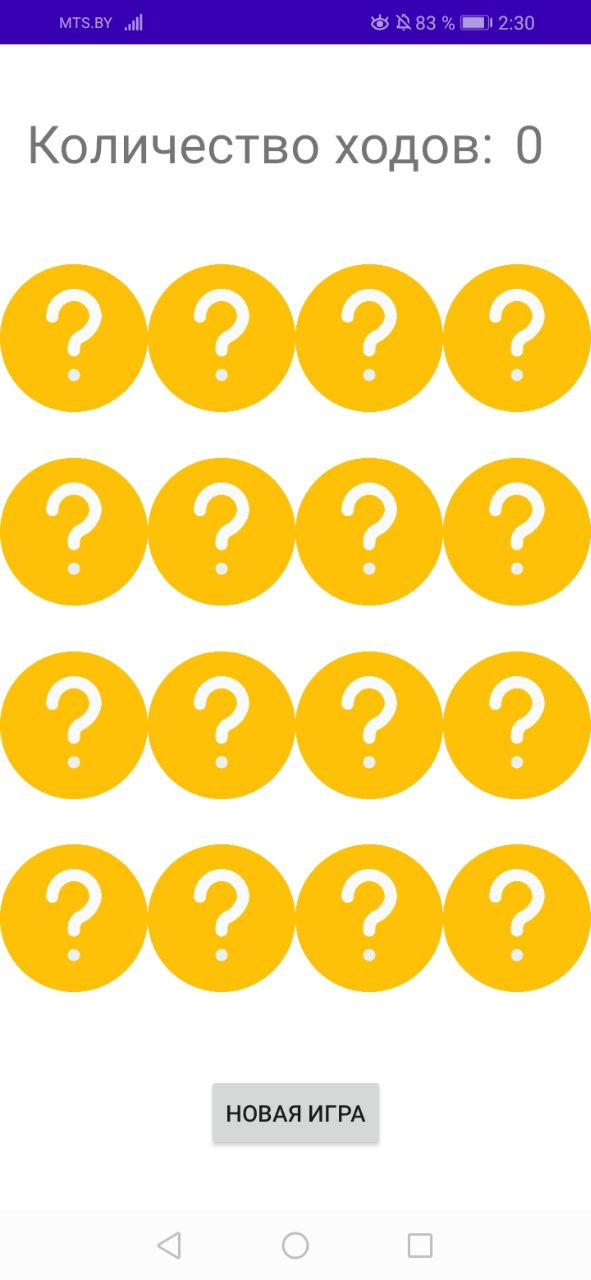
\includegraphics[height=6cm]
                {_assets/step_1.jpg}
            \caption{шаг 1}
            \label{fig:step_1}
        \end{minipage}
        \begin{minipage}{0.15\textwidth}
            \centering
            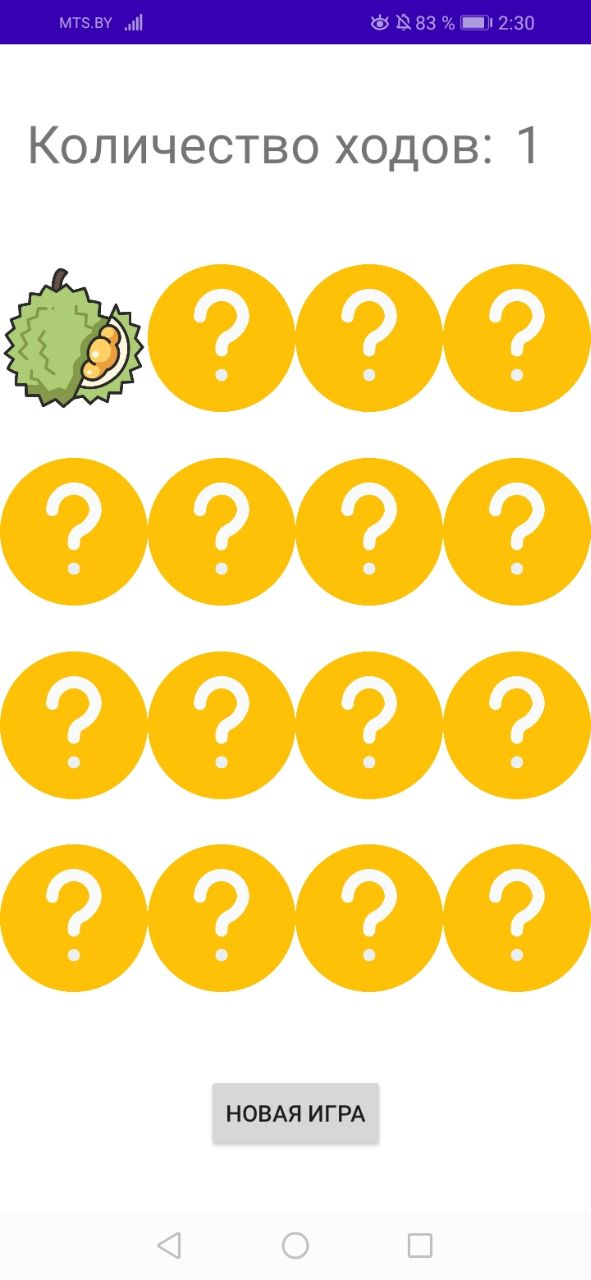
\includegraphics[height=6cm]
                {_assets/step_2.jpg}
            \caption{шаг 2}
            \label{fig:step_2}
        \end{minipage}
        \begin{minipage}{0.15\textwidth}
            \centering
            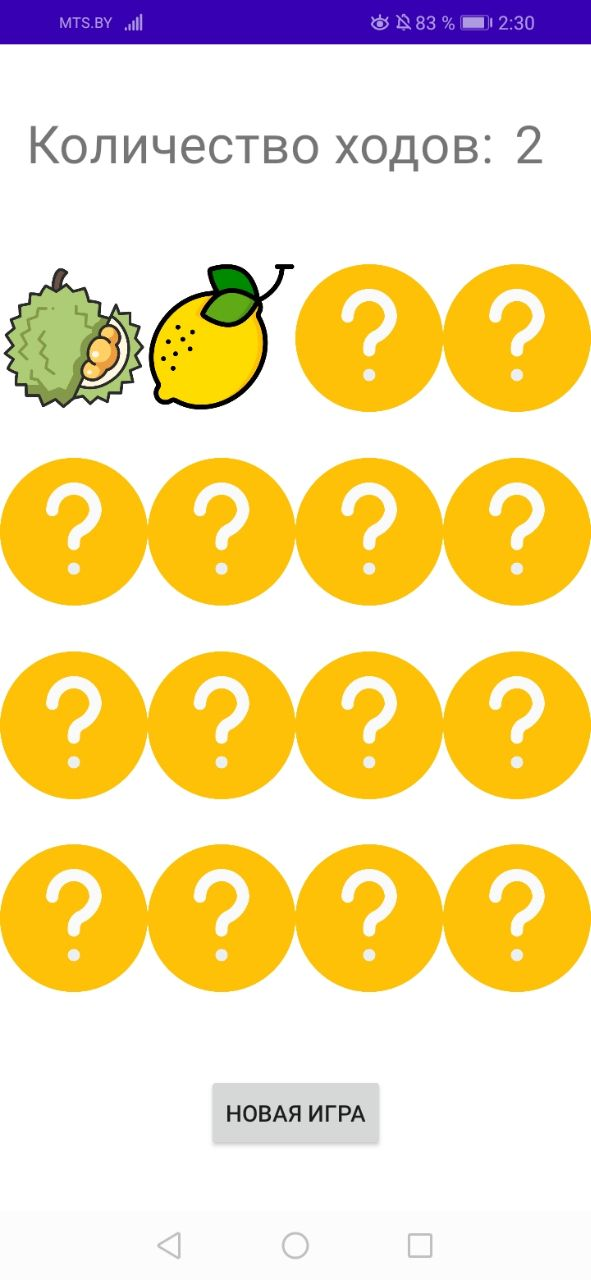
\includegraphics[height=6cm]
                {_assets/step_3.jpg}
            \caption{шаг 3}
            \label{fig:step_3}
        \end{minipage}
        \begin{minipage}{0.15\textwidth}
            \centering
            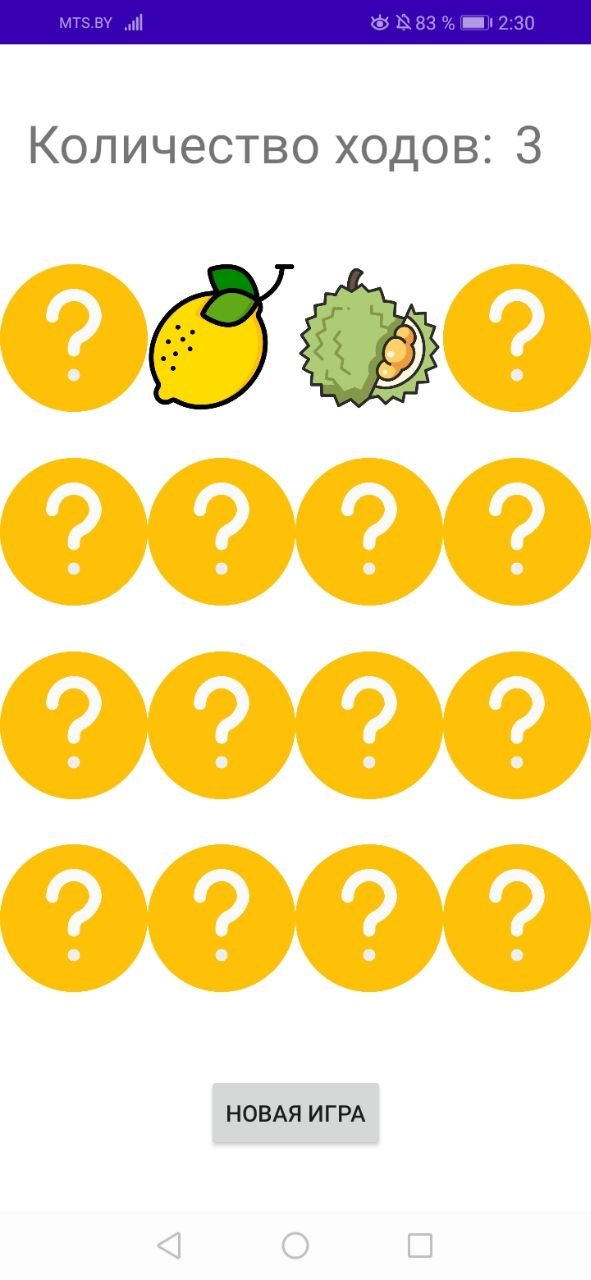
\includegraphics[height=6cm]
                {_assets/step_4.jpg}
            \caption{шаг 4}
            \label{fig:step_4}
        \end{minipage}
        \begin{minipage}{0.15\textwidth}
            \centering
            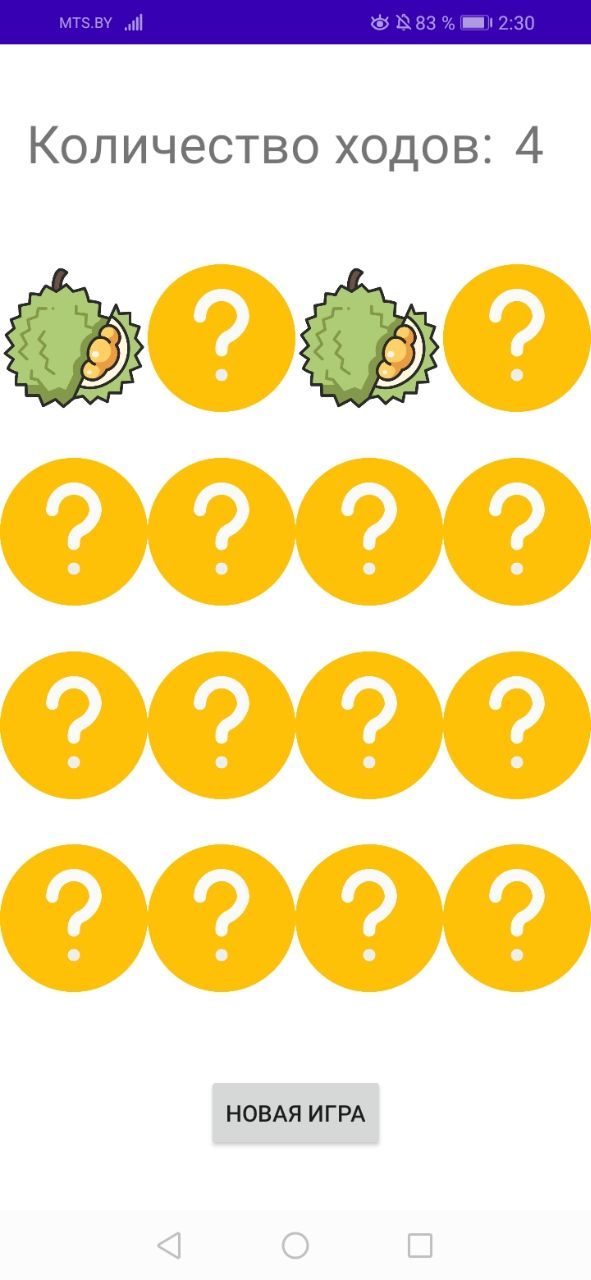
\includegraphics[height=6cm]
                {_assets/step_5.jpg}
            \caption{шаг 5}
            \label{fig:step_5}
        \end{minipage}
        \begin{minipage}{0.15\textwidth}
            \centering
            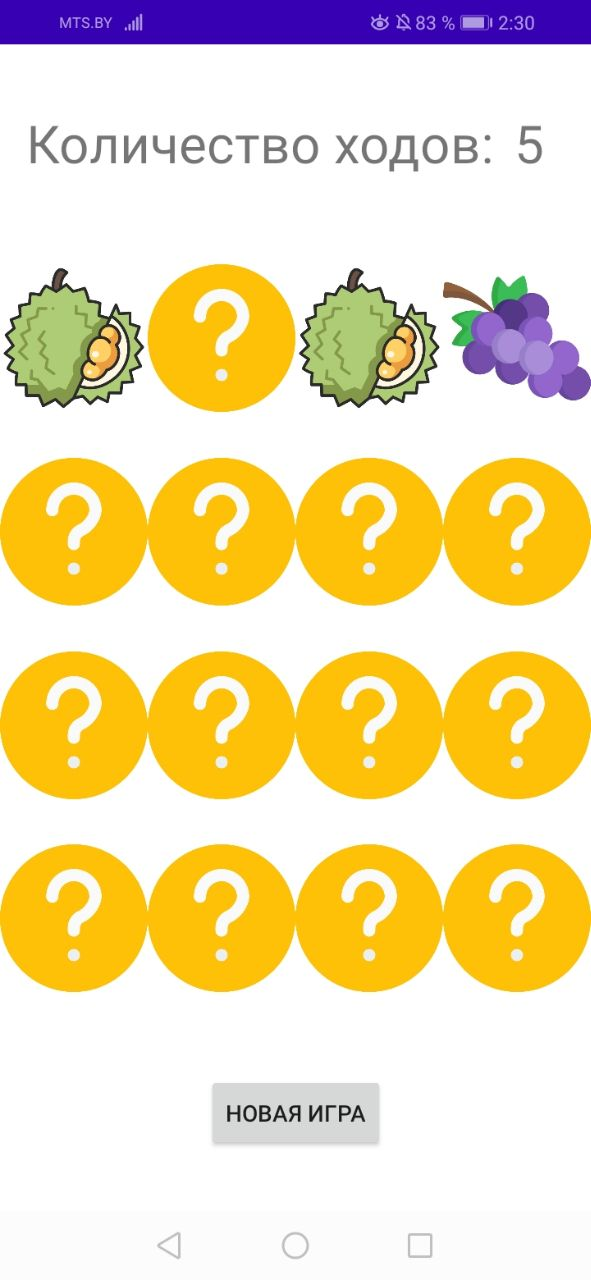
\includegraphics[height=6cm]
                {_assets/step_6.jpg}
            \caption{шаг 6}
            \label{fig:step_6}
        \end{minipage}
    \end{figure}

    \begin{figure}[!h]
        \centering
        \begin{minipage}{0.15\textwidth}
            \centering
            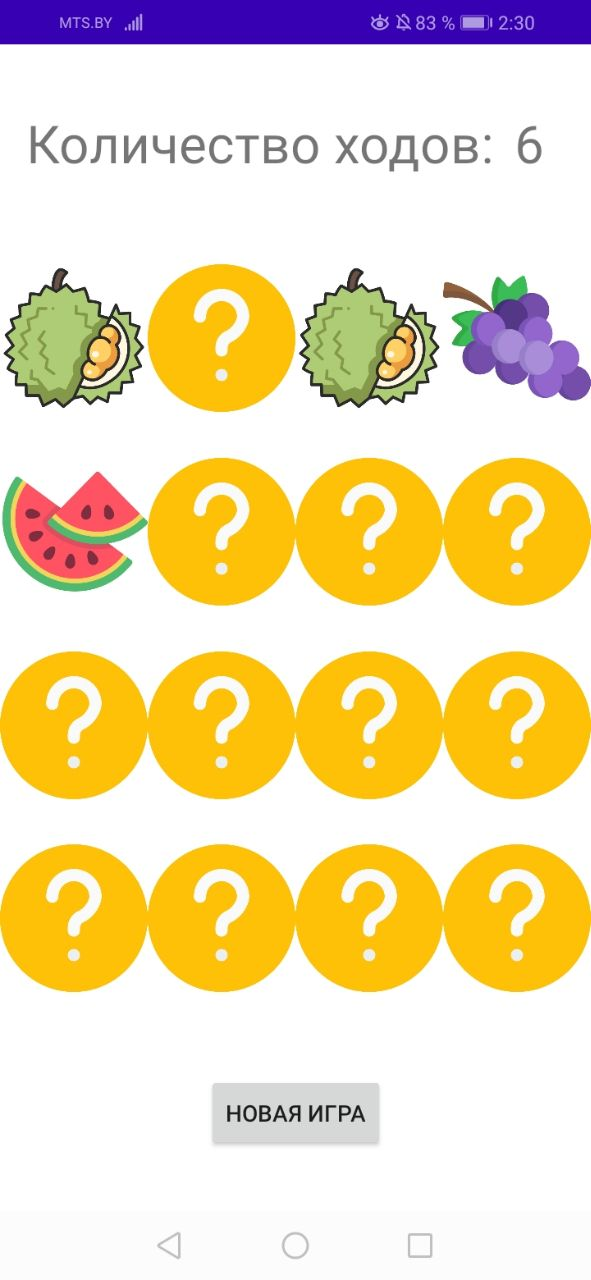
\includegraphics[height=6cm]
                {_assets/step_7.jpg}
            \caption{шаг 7}
            \label{fig:step_7}
        \end{minipage}
        \begin{minipage}{0.15\textwidth}
            \centering
            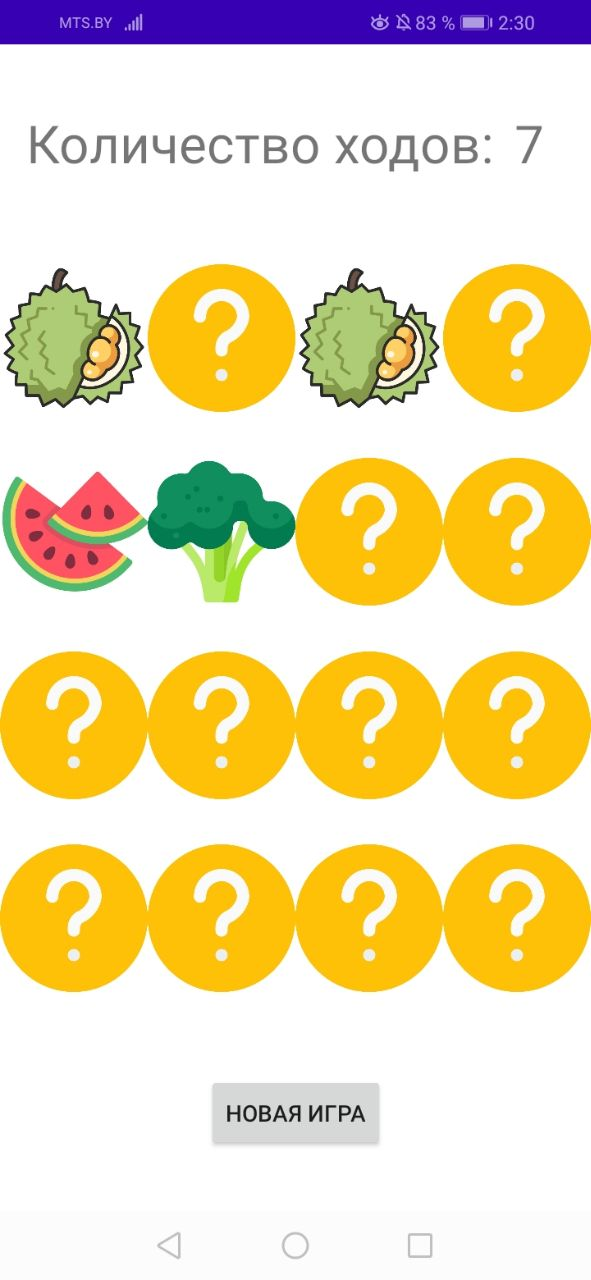
\includegraphics[height=6cm]
                {_assets/step_8.jpg}
            \caption{шаг 8}
            \label{fig:step_8}
        \end{minipage}
        \begin{minipage}{0.15\textwidth}
            \centering
            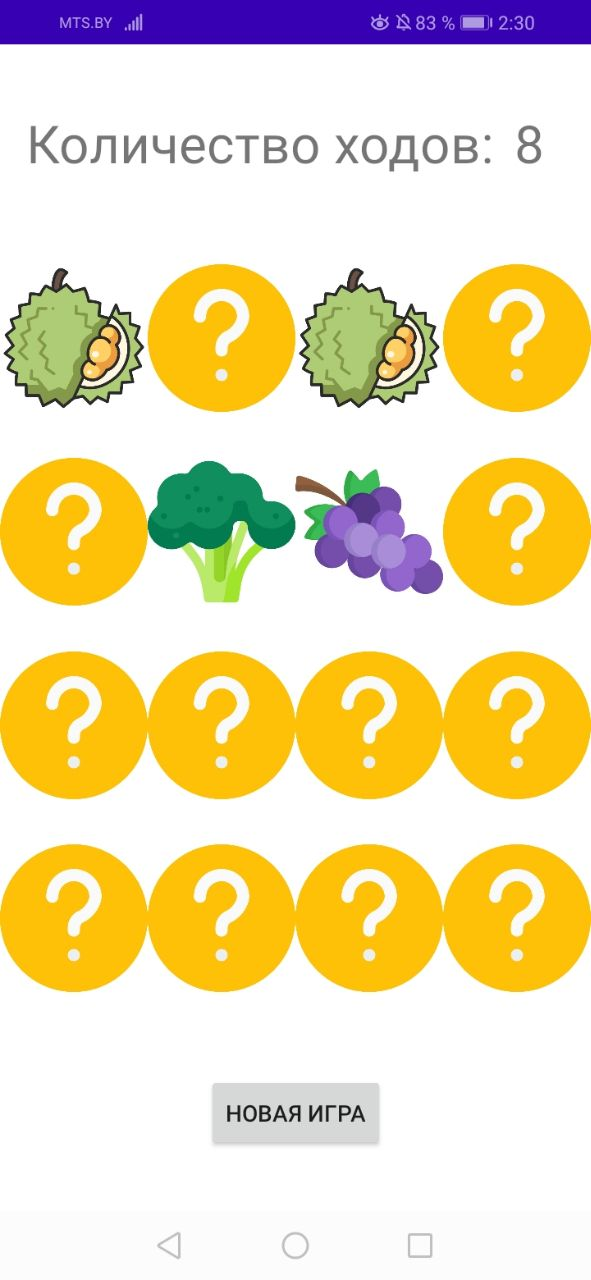
\includegraphics[height=6cm]
                {_assets/step_9.jpg}
            \caption{шаг 9}
            \label{fig:step_9}
        \end{minipage}
        \begin{minipage}{0.15\textwidth}
            \centering
            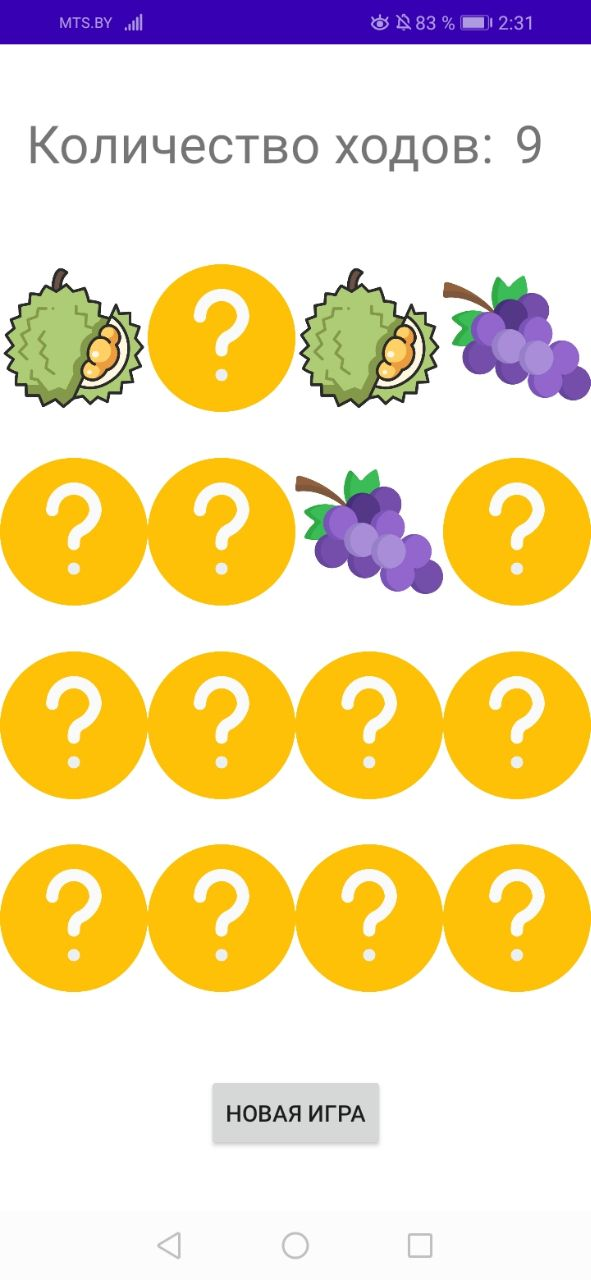
\includegraphics[height=6cm]
                {_assets/step_10.jpg}
            \caption{шаг 10}
            \label{fig:step_10}
        \end{minipage}
        \begin{minipage}{0.15\textwidth}
            \centering
            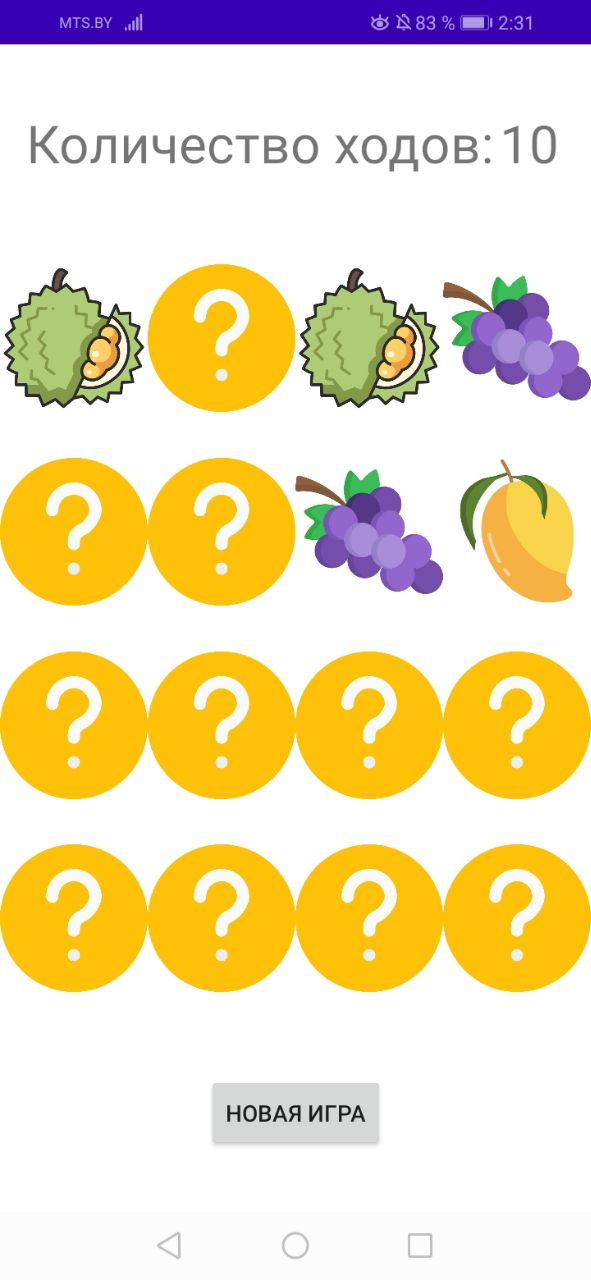
\includegraphics[height=6cm]
                {_assets/step_11.jpg}
            \caption{шаг 11}
            \label{fig:step_11}
        \end{minipage}
        \begin{minipage}{0.15\textwidth}
            \centering
            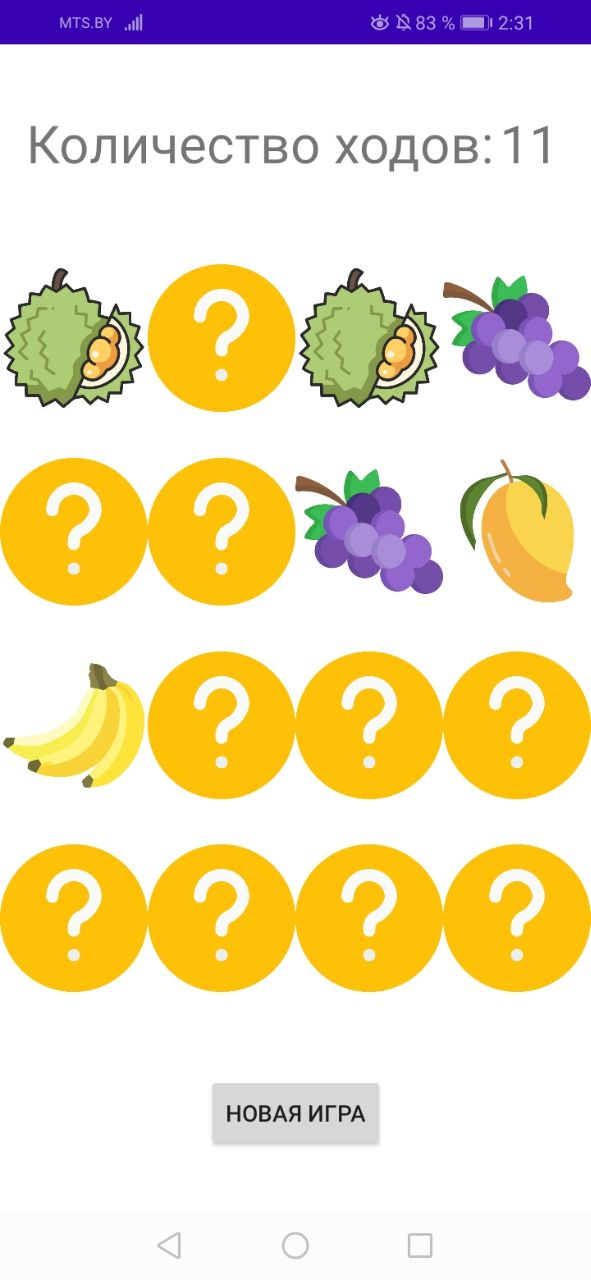
\includegraphics[height=6cm]
                {_assets/step_12.jpg}
            \caption{шаг 12}
            \label{fig:step_12}
        \end{minipage}
    \end{figure}

    \begin{figure}[!h]
        \centering
        \begin{minipage}{0.15\textwidth}
            \centering
            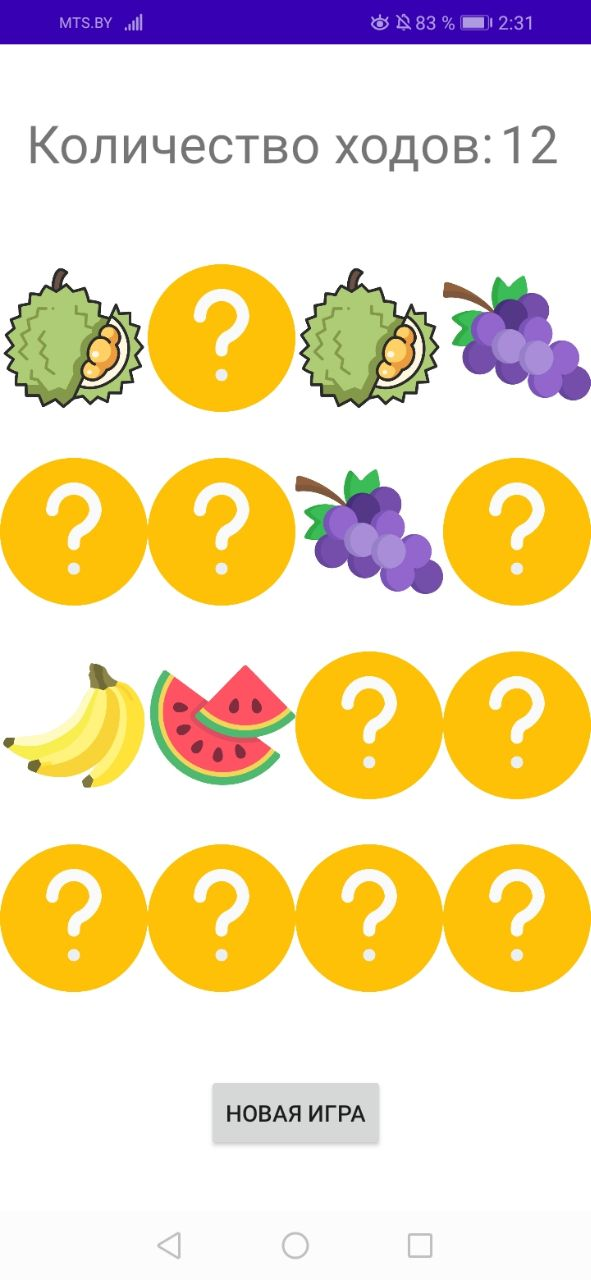
\includegraphics[height=6cm]
                {_assets/step_13.jpg}
            \caption{шаг 13}
            \label{fig:step_13}
        \end{minipage}
        \begin{minipage}{0.15\textwidth}
            \centering
            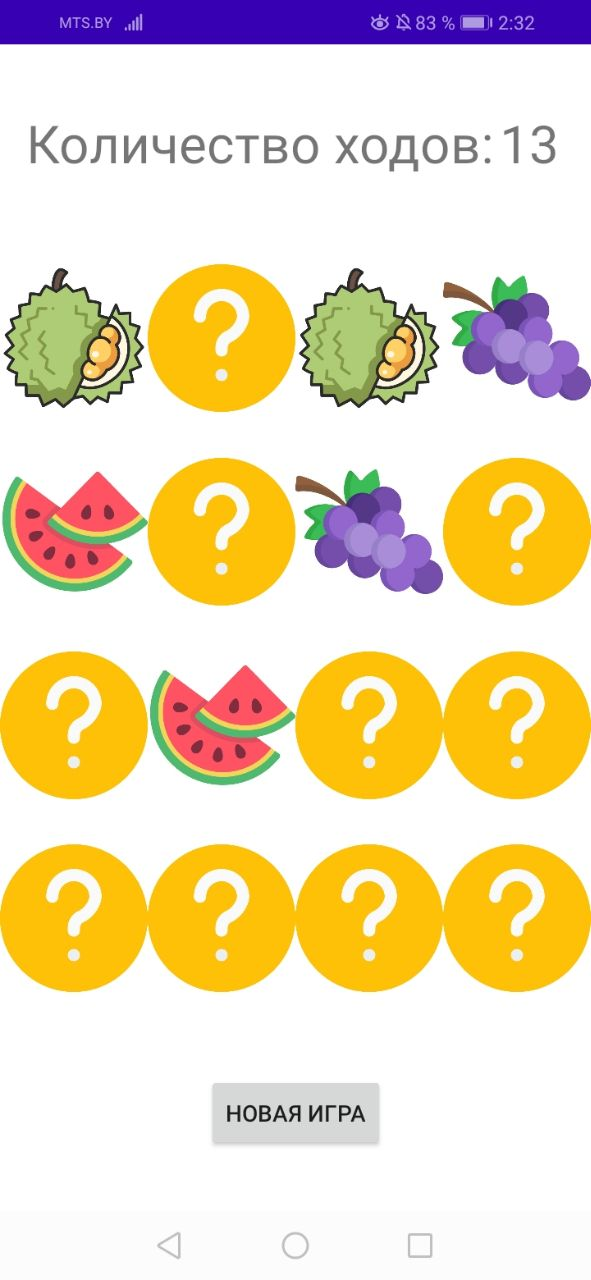
\includegraphics[height=6cm]
                {_assets/step_14.jpg}
            \caption{шаг 14}
            \label{fig:step_14}
        \end{minipage}
        \begin{minipage}{0.15\textwidth}
            \centering
            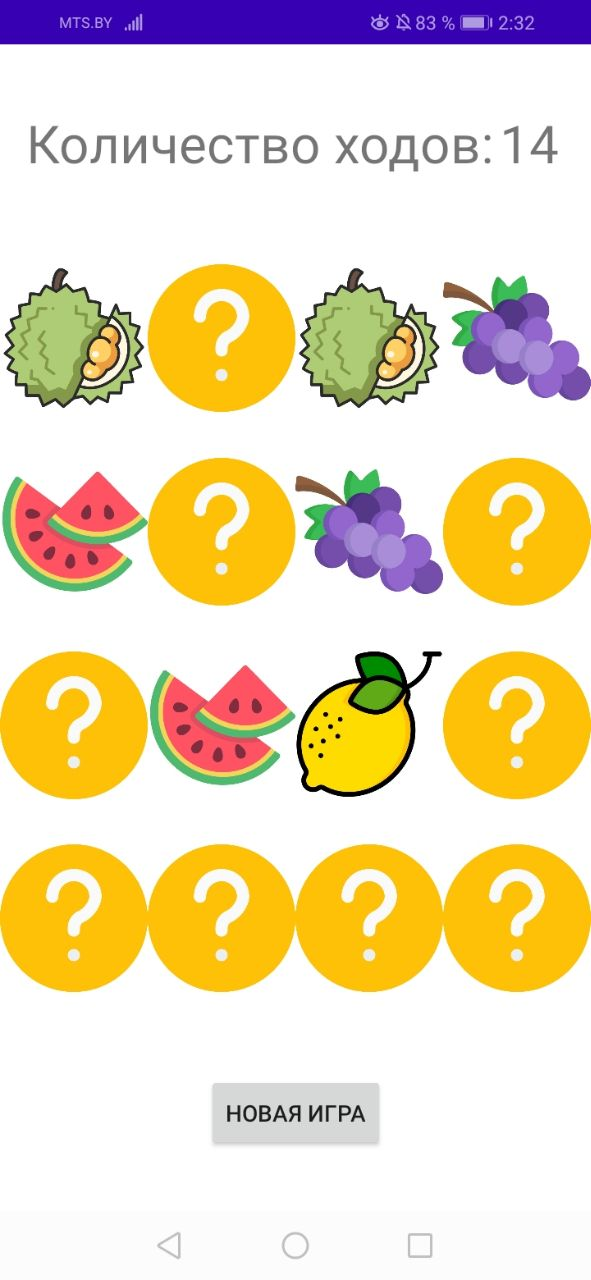
\includegraphics[height=6cm]
                {_assets/step_15.jpg}
            \caption{шаг 15}
            \label{fig:step_15}
        \end{minipage}
        \begin{minipage}{0.15\textwidth}
            \centering
            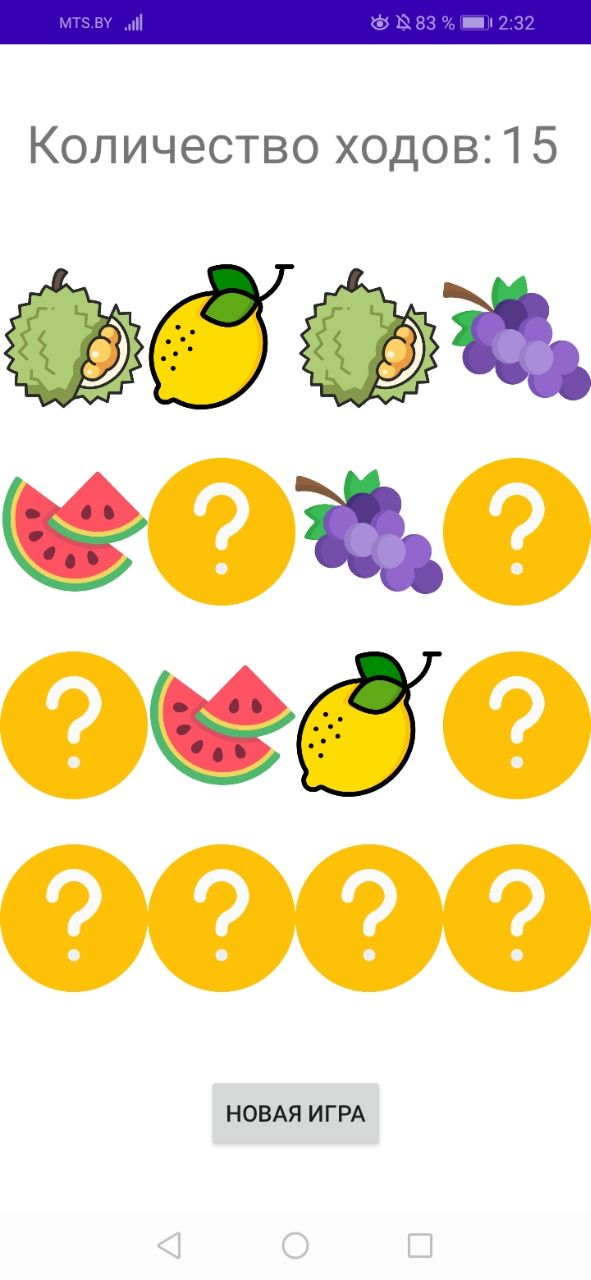
\includegraphics[height=6cm]
                {_assets/step_16.jpg}
            \caption{шаг 16}
            \label{fig:step_16}
        \end{minipage}
        \begin{minipage}{0.15\textwidth}
            \centering
            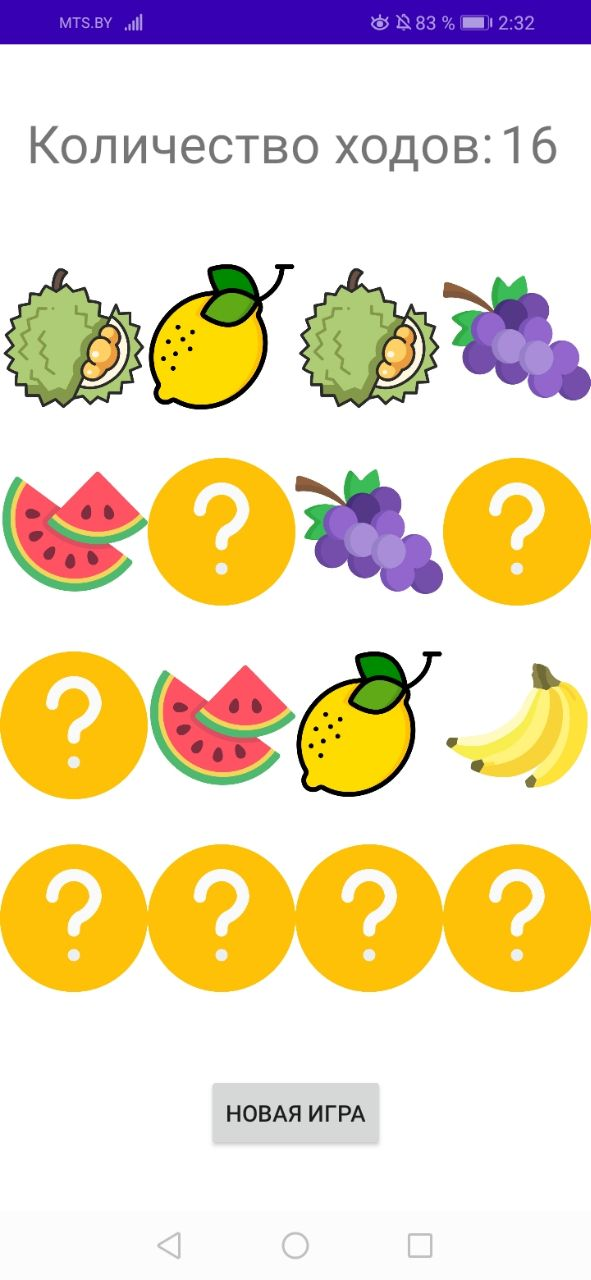
\includegraphics[height=6cm]
                {_assets/step_17.jpg}
            \caption{шаг 17}
            \label{fig:step_17}
        \end{minipage}
        \begin{minipage}{0.15\textwidth}
            \centering
            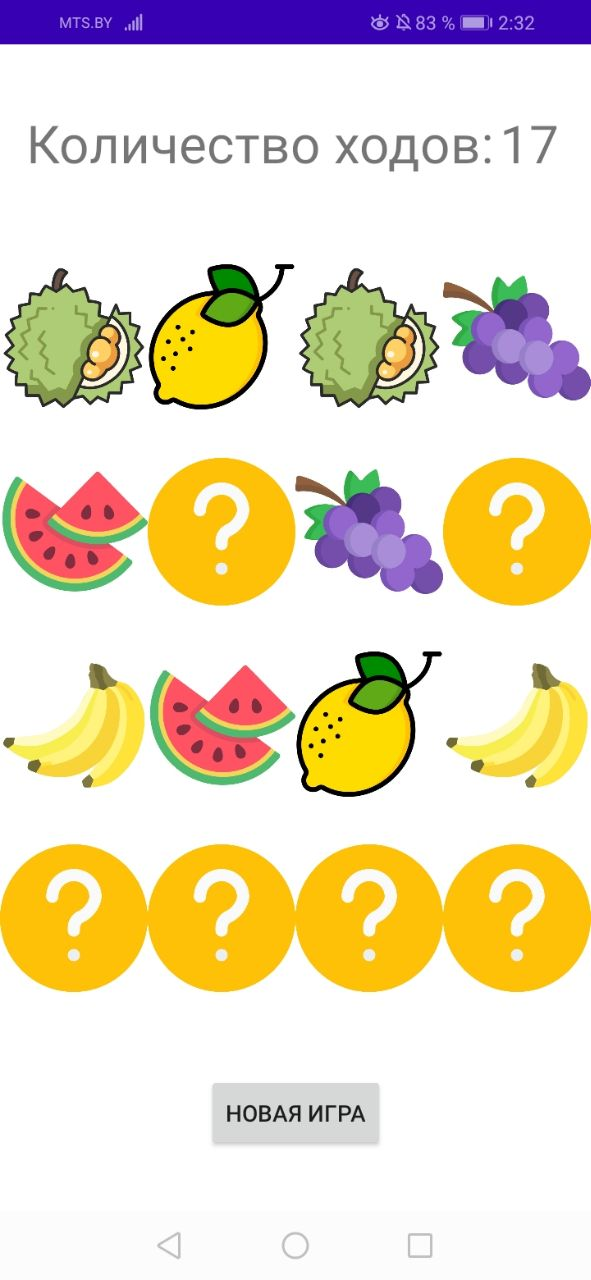
\includegraphics[height=6cm]
                {_assets/step_18.jpg}
            \caption{шаг 18}
            \label{fig:step_18}
        \end{minipage}
    \end{figure}
    
    \begin{figure}[!h]
        \centering
        \begin{minipage}{0.15\textwidth}
            \centering
            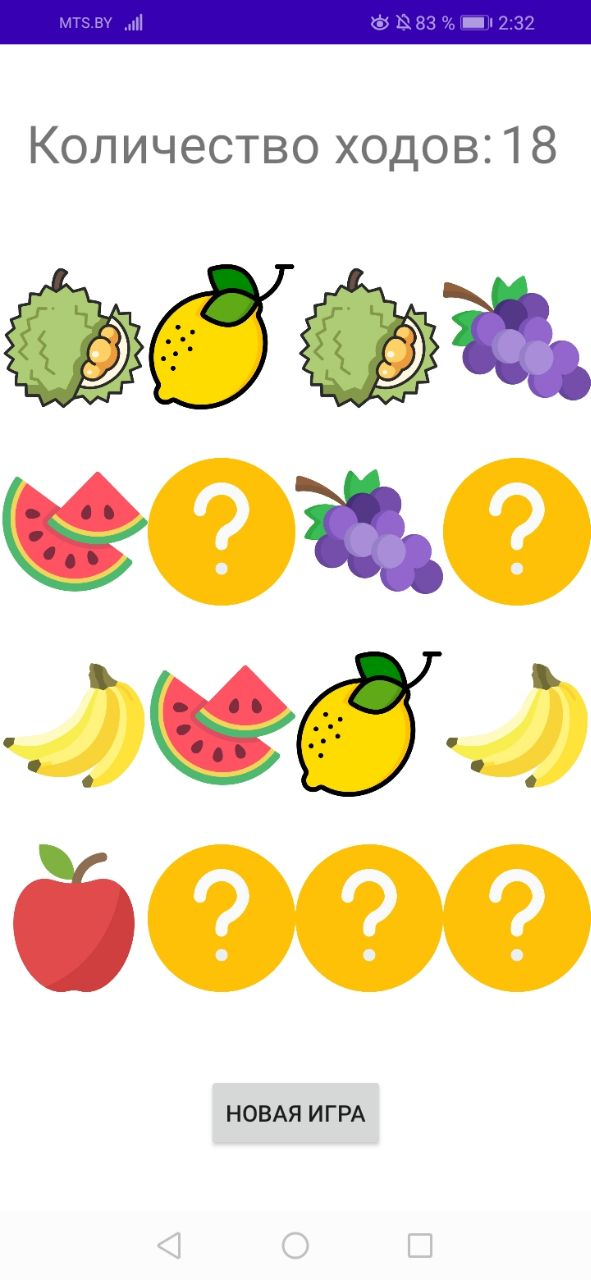
\includegraphics[height=6cm]
                {_assets/step_19.jpg}
            \caption{шаг 19}
            \label{fig:step_19}
        \end{minipage}
        \begin{minipage}{0.15\textwidth}
            \centering
            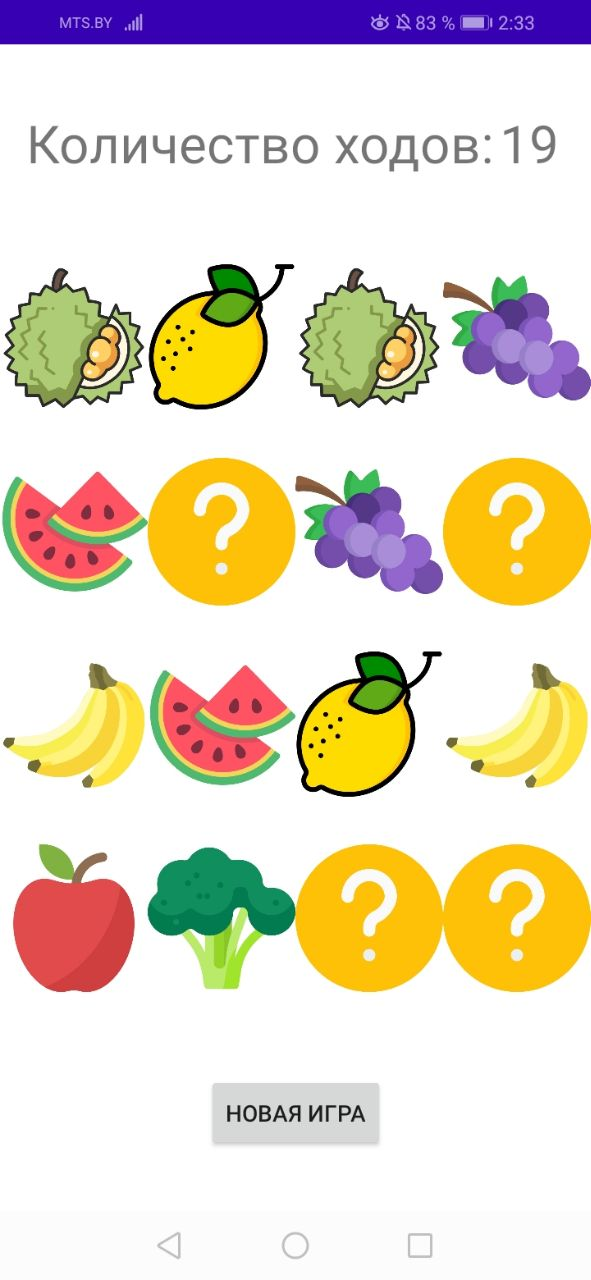
\includegraphics[height=6cm]
                {_assets/step_20.jpg}
            \caption{шаг 20}
            \label{fig:step_20}
        \end{minipage}
        \begin{minipage}{0.15\textwidth}
            \centering
            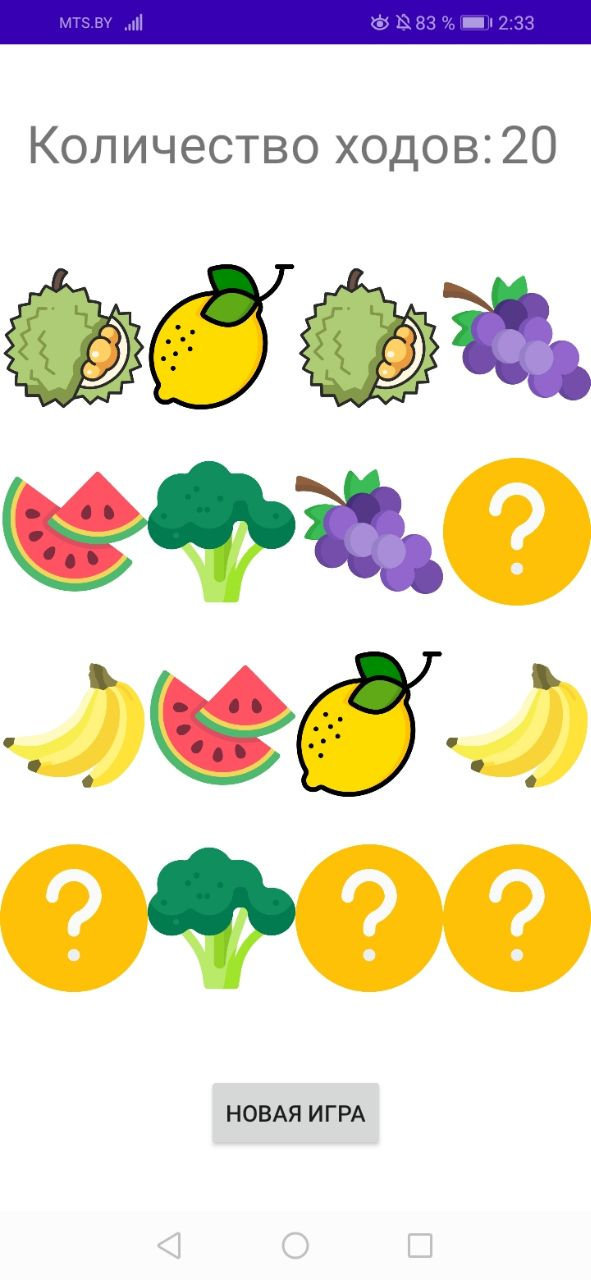
\includegraphics[height=6cm]
                {_assets/step_21.jpg}
            \caption{шаг 21}
            \label{fig:step_21}
        \end{minipage}
        \begin{minipage}{0.15\textwidth}
            \centering
            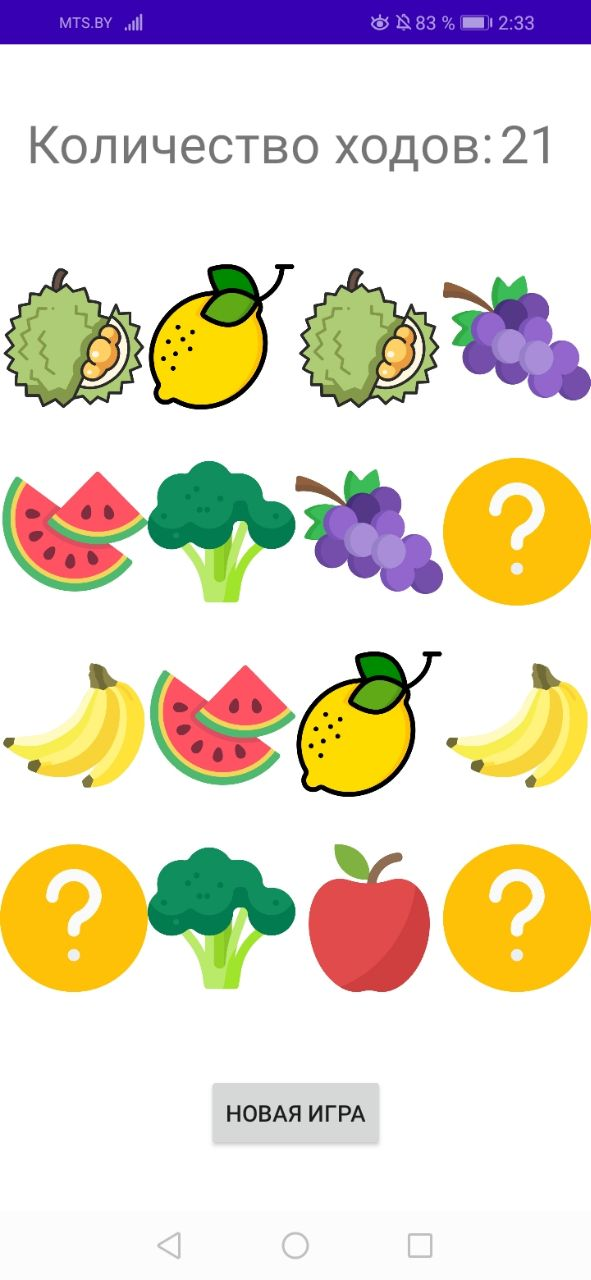
\includegraphics[height=6cm]
                {_assets/step_22.jpg}
            \caption{шаг 22}
            \label{fig:step_22}
        \end{minipage}
        \begin{minipage}{0.15\textwidth}
            \centering
            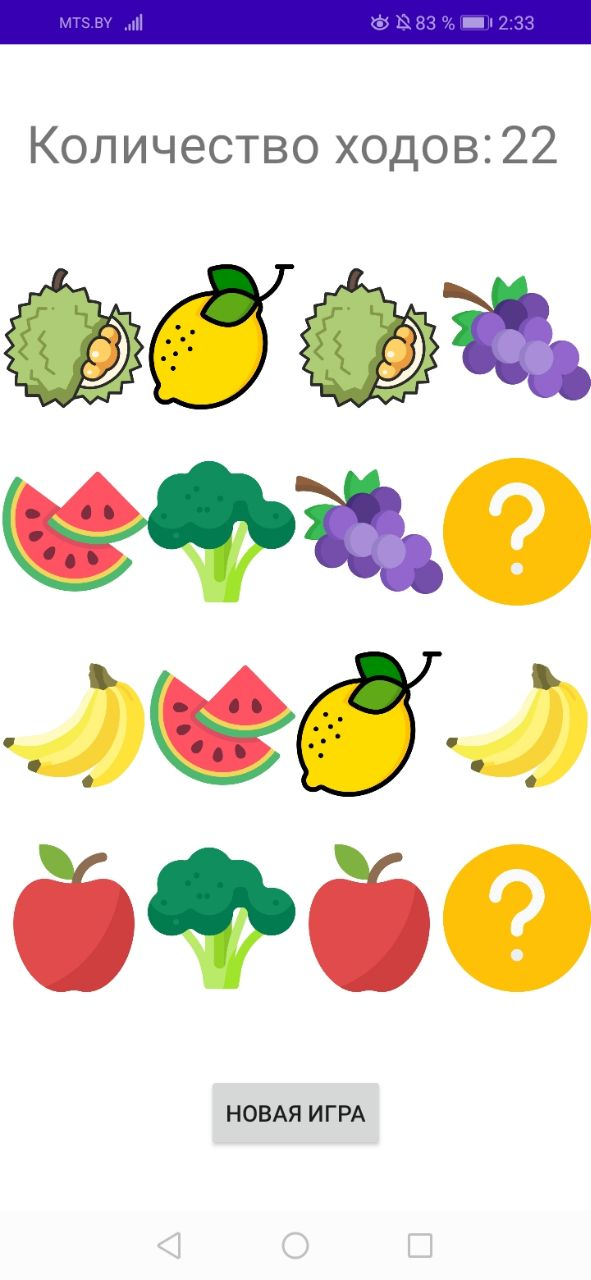
\includegraphics[height=6cm]
                {_assets/step_23.jpg}
            \caption{шаг 23}
            \label{fig:step_23}
        \end{minipage}
        \begin{minipage}{0.15\textwidth}
            \centering
            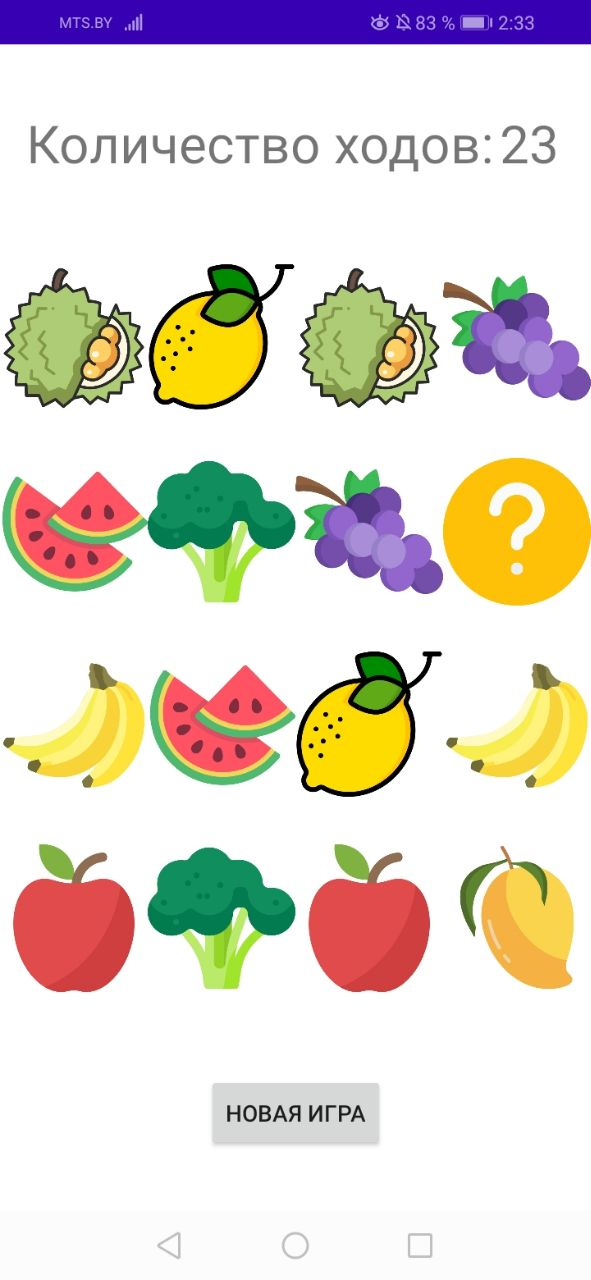
\includegraphics[height=6cm]
                {_assets/step_24.jpg}
            \caption{шаг 24}
            \label{fig:step_24}
        \end{minipage}
    \end{figure}

    \begin{figure}[!h]
        \centering
        \begin{minipage}{0.15\textwidth}
            \centering
            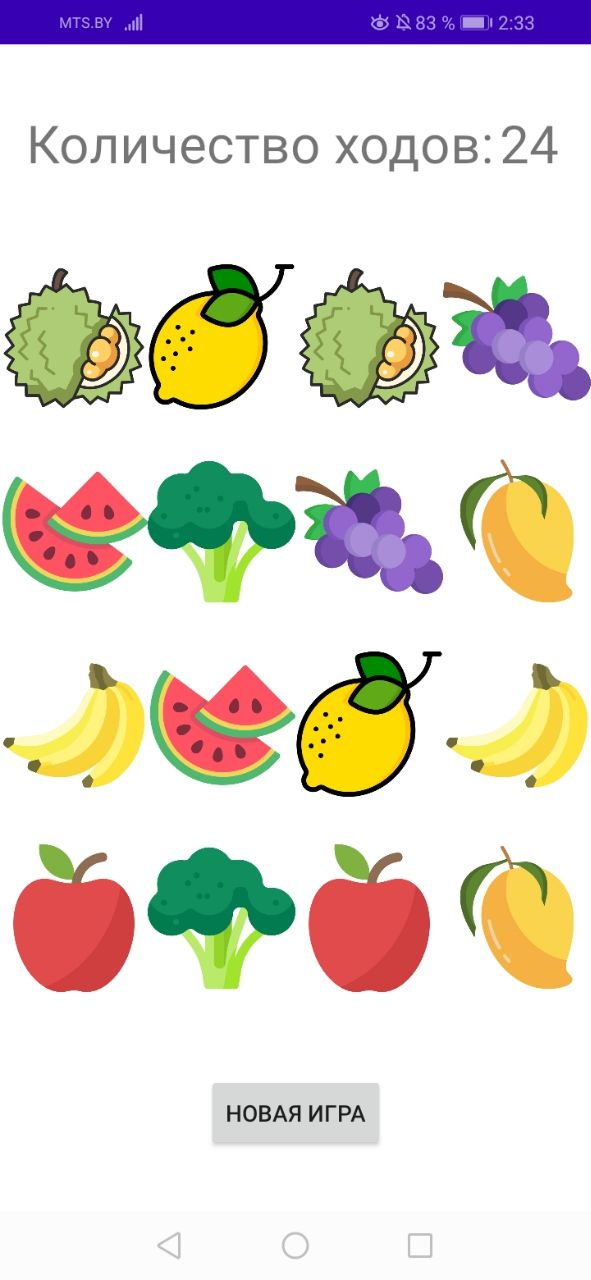
\includegraphics[height=6cm]
                {_assets/step_25.jpg}
            \caption{шаг 25}
            \label{fig:step_25}
        \end{minipage}
        \begin{minipage}{0.15\textwidth}
            \centering
            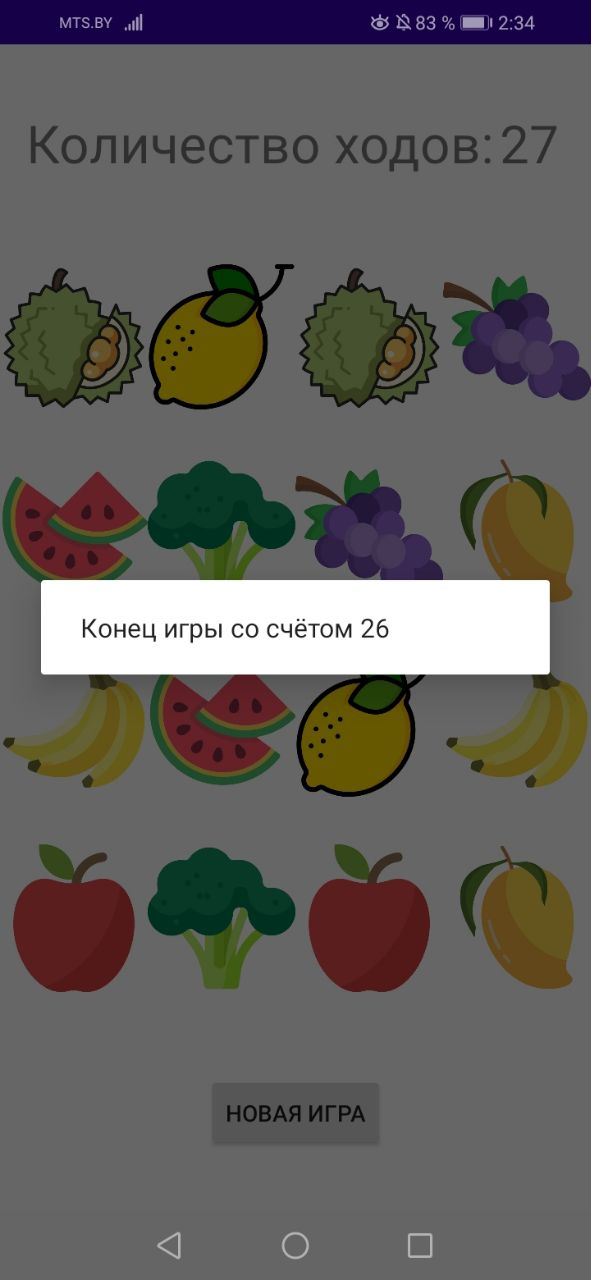
\includegraphics[height=6cm]
                {_assets/step_26.jpg}
            \caption{шаг 26}
            \label{fig:step_26}
        \end{minipage}
        \begin{minipage}{0.15\textwidth}
            \centering
            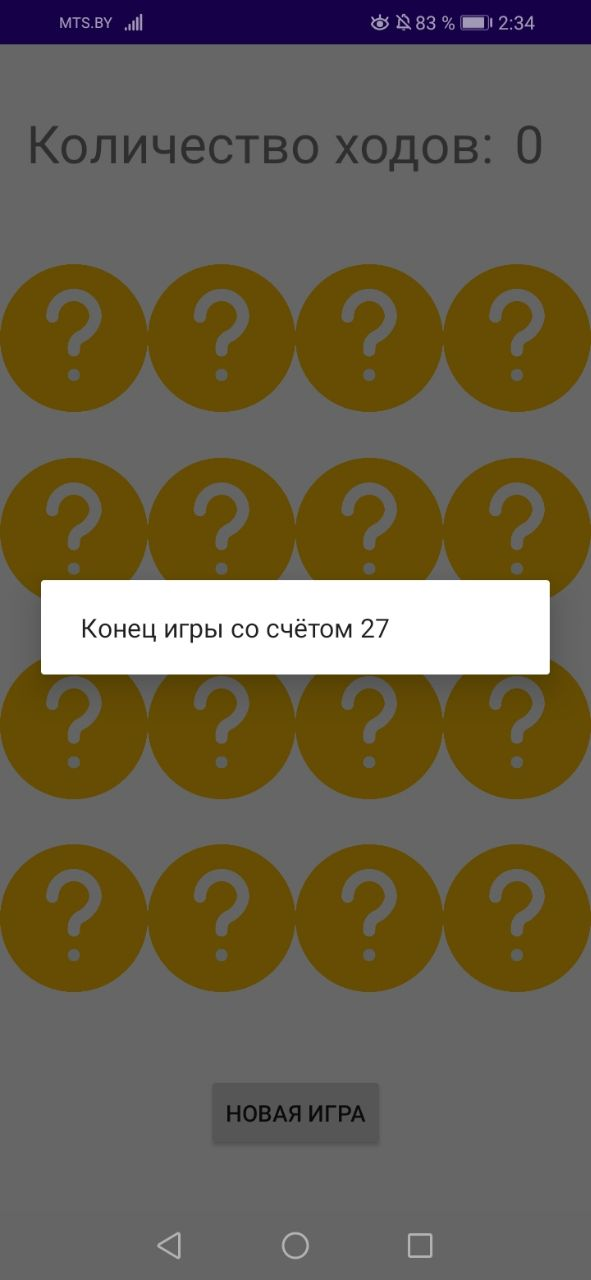
\includegraphics[height=6cm]
                {_assets/step_27.jpg}
            \caption{шаг 27}
            \label{fig:step_27}
        \end{minipage}
    \end{figure}

    % \begin{figure}[!h]
    %     \centering
    %     \includegraphics[height=11cm]
    %         {_assets/gpi_RaitingImages.jpg}
    %     \caption{Приложение <<RaitingImages>>}
    %     \label{fig:gpi_hit}
    % \end{figure}

    \newpage

    \lstinputlisting[language=xml, name=app/src/main/res/values/strings.xml]
        {../gpi_src/gpi_rpodms6_lab4__memory_game/app/src/main/res/values/strings.xml}

    \lstinputlisting[language=xml, name=app/src/main/res/layout/activity_main.xml]
        {../gpi_src/gpi_rpodms6_lab4__memory_game/app/src/main/res/layout/activity_main.xml}

    \lstinputlisting[language=java, name=app/src/main/java/.../MainActivity.java]
        {../gpi_src/gpi_rpodms6_lab4__memory_game/app/src/main/java/io/github/Pavel_Innokentevich_Galanin/gpi_rpodms6_lab4__memory_game/MainActivity.java}

    % \subparagraph{} \hspace{0pt}

    % \textbf{Вывод}: Разработал дизайн приложения <<RaitingImages>>.
    % Использовали LinearLayout, RelativeLayout и FrameLayout для слоев.
    % Задали верхнему тегу задний фон.
    % Создали EditText с текстом подсказкой, занеся в string.xml. Поменяли цвет EditText.
    % Создали кнопку Button c текстом из string.xml.
    % Создали ImageView, указан ссылку на картинку и contentDescription.

    % \newpage

    % = = = = = = = =
    \paragraph{} \textbf{Список использованных источников} 
    % \addcontentsline{toc}{section}{СПИСОК ИСПОЛЬЗОВАННЫХ ИСТОЧНИКОВ}
    % \section*{Список использованных источников}

    \begin{enumerate}
        \item[1.] литературу не использовал. Создавал свою игру.
    \end{enumerate}
\end{document}
